\subsection{Fenómenos ondulatorios}

En la unidad anterior \ref{sec:waves_analisys} vimos de forma superficial algunos de los fenómenos ondulatorios. El único fenómeno que vimos con detalle fue la reflexión.

Ahora vamos a ver los fenómenos ondulatorios que aplican tanto a ondas mecánicas (como el sonido o las ondas en una cuerda) como a ondas electromagnéticas (como la luz o las microondas), con ciertas particularidades en cada caso.

En general los fenómenos ondulatorios son:

\begin{itemize}
  \item Reflexión
  \item Refracción
  \item Interferencia
  \item Difracción
  \item Polarización
\end{itemize}

\subsubsection{Reflexión}
\label{sec:reflection}

\begin{wrapfigure}{r}{0.24\textwidth}
  \centering
  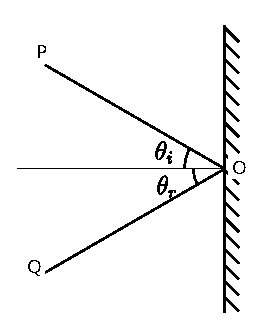
\includegraphics[width=\linewidth]{reflection_angles.pdf}
  \caption{Ángulos de reflexión}
  \label{fig:reflection_angles}
\end{wrapfigure}
La reflexión es el cambio en la dirección de propagación de una onda cuando choca contra una superficie y retorna al medio original.

La reflexión obedece a las siguientes reglas: el rayo incidente, el rayo reflejado y la normal a la superficie están en el mismo plano, y para ondas que inciden sobre una superficie lisa (o un diferencial de superficie considerado liso) el ángulo de incidencia (\(\theta_i\)) es igual al ángulo de reflexión (\(\theta_r\)):
\[
  \theta_i = \theta_r
\]
Ejemplos:
\begin{itemize}
  \item Una onda en una cuerda que regresa al encontrar un extremo fijo.
  \item Un rayo de luz reflejándose en un espejo plano.
  \item Un eco producido por una onda sonora al rebotar en una pared.
\end{itemize}

\begin{wrapfigure}{l}{0.3\textwidth}
  \centering
  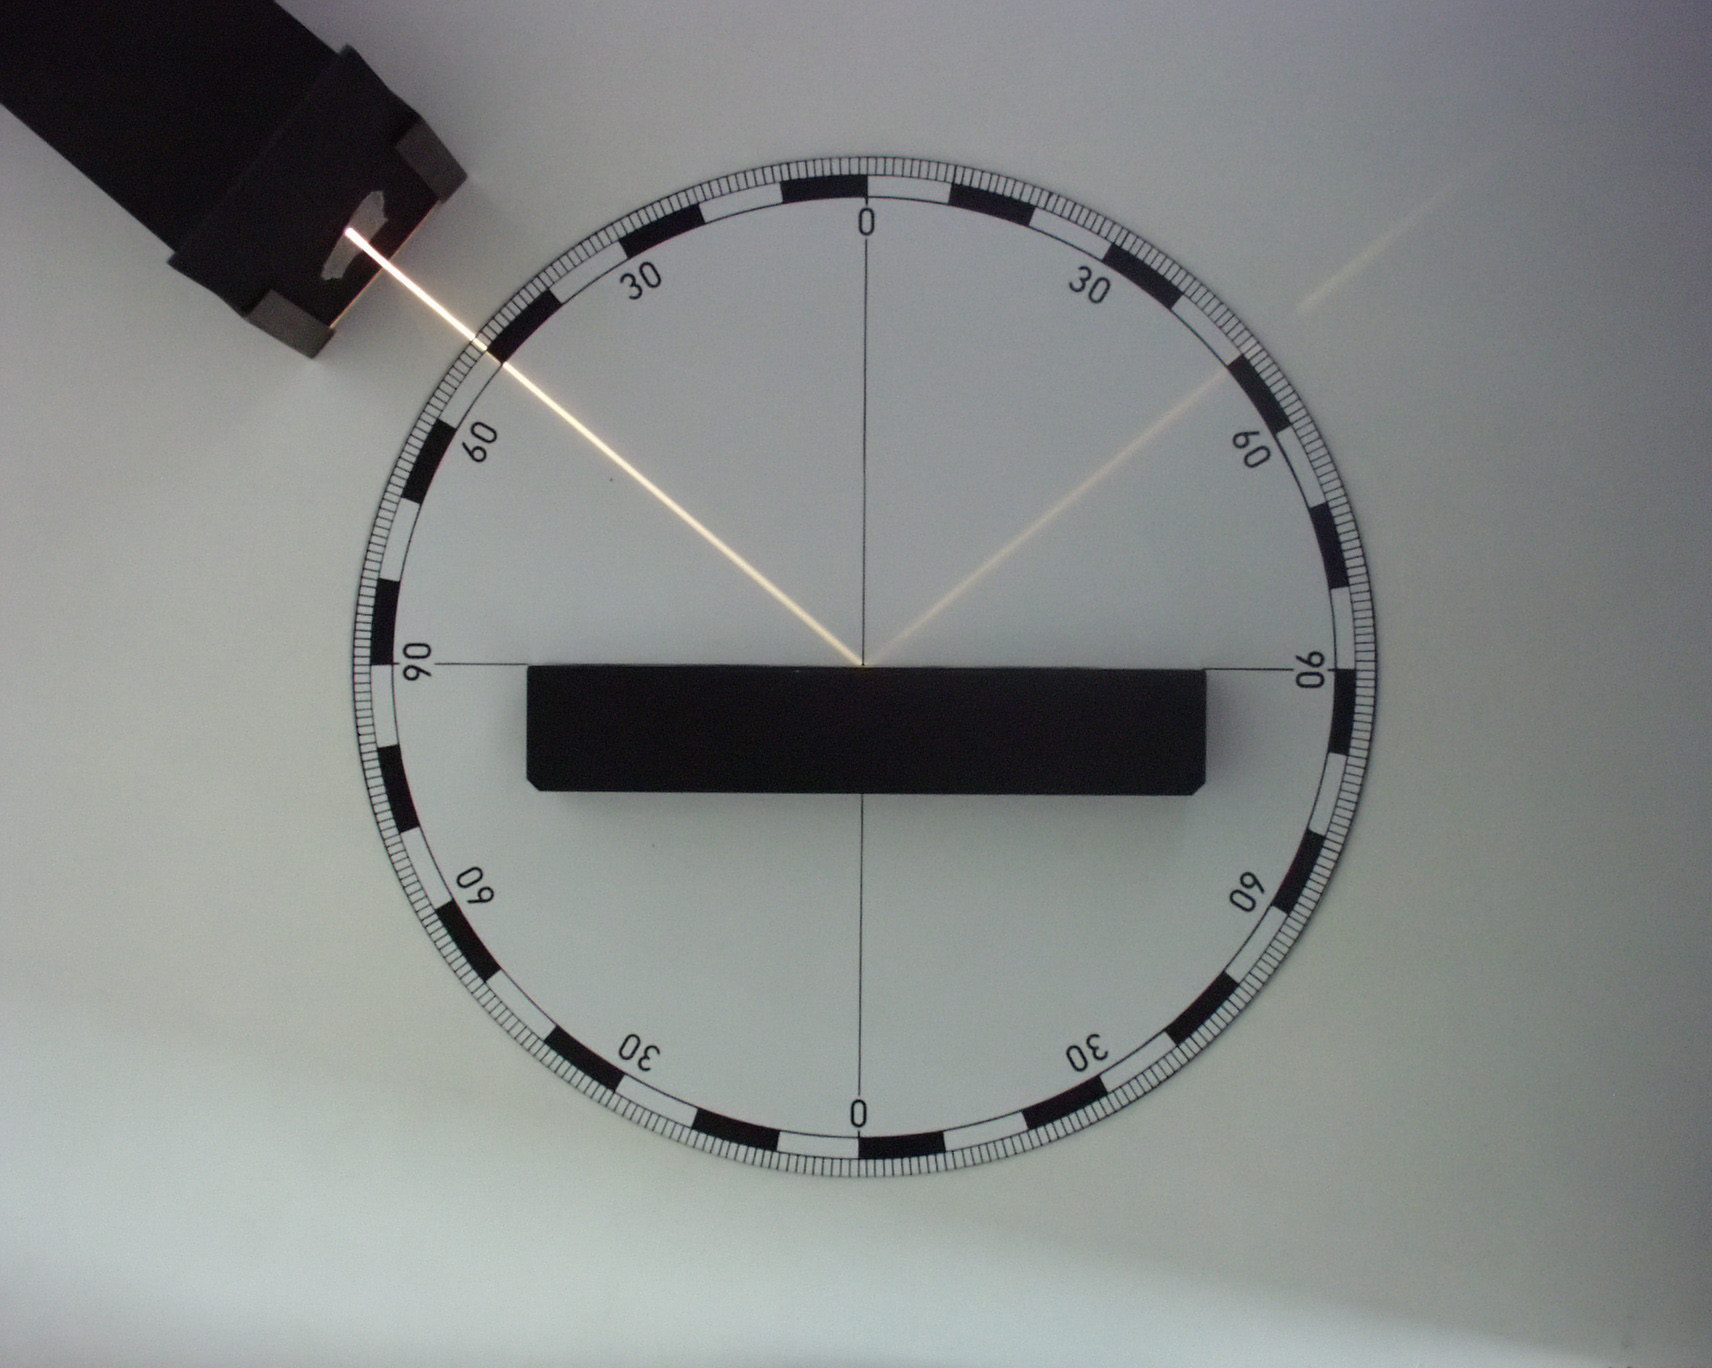
\includegraphics[width=\linewidth]{reflection_example.jpg}
  \caption{Reflexión de un haz de luz.}
  \label{fig:reflexion}
\end{wrapfigure}
Podemos encontrar dos tipos de reflexión según la superficie: reflexión \textbf{difusa} y reflexión \textbf{especular}. La reflexión difusa ocurre cuando la superficie es rugosa o desglosada, y la reflexión especular ocurre cuando la superficie es lisa.

En ondas mecánicas (como en cuerdas), la fase puede invertirse si la onda rebota en un medio más rígido (más denso). Se vió un ejemplo de esto con más detalle en la sección \ref{sec:waves_analisys}. 

En el caso de la luz (y en general cualquier onda electromagnética) también \textbf{puede invertir su fase} al reflejarse, dependiendo de las propiedades ópticas del medio en el que ocurre la reflexión.

La inversión de fase ocurre cuando una onda electromagnética se refleja en la superficie de \textbf{un medio con mayor índice de refracción que el medio del que proviene}. En ese caso, la onda reflejada experimenta un cambio de fase de \(\pi\) radianes (\(180^\circ\)).

En otras palabras, si la luz pasa de un medio con índice de refracción \(n_1\) a otro con \(n_2\), entonces:
\begin{itemize}
  \item Si \(n_2 > n_1\), la onda reflejada sufre un cambio de fase de \(\pi\) radianes (\(180^\circ\)).
  \item Si \(n_2 < n_1\), la onda reflejada no sufre un cambio de fase.
\end{itemize}

\subsubsection{Refracción y la ley de Snell}

La refracción es el fenómeno por el cual una onda electromagnética cambia de dirección y velocidad al pasar de un medio material a otro con diferente índice de refracción.

\begin{wrapfigure}{r}{0.3\textwidth}
  \centering
  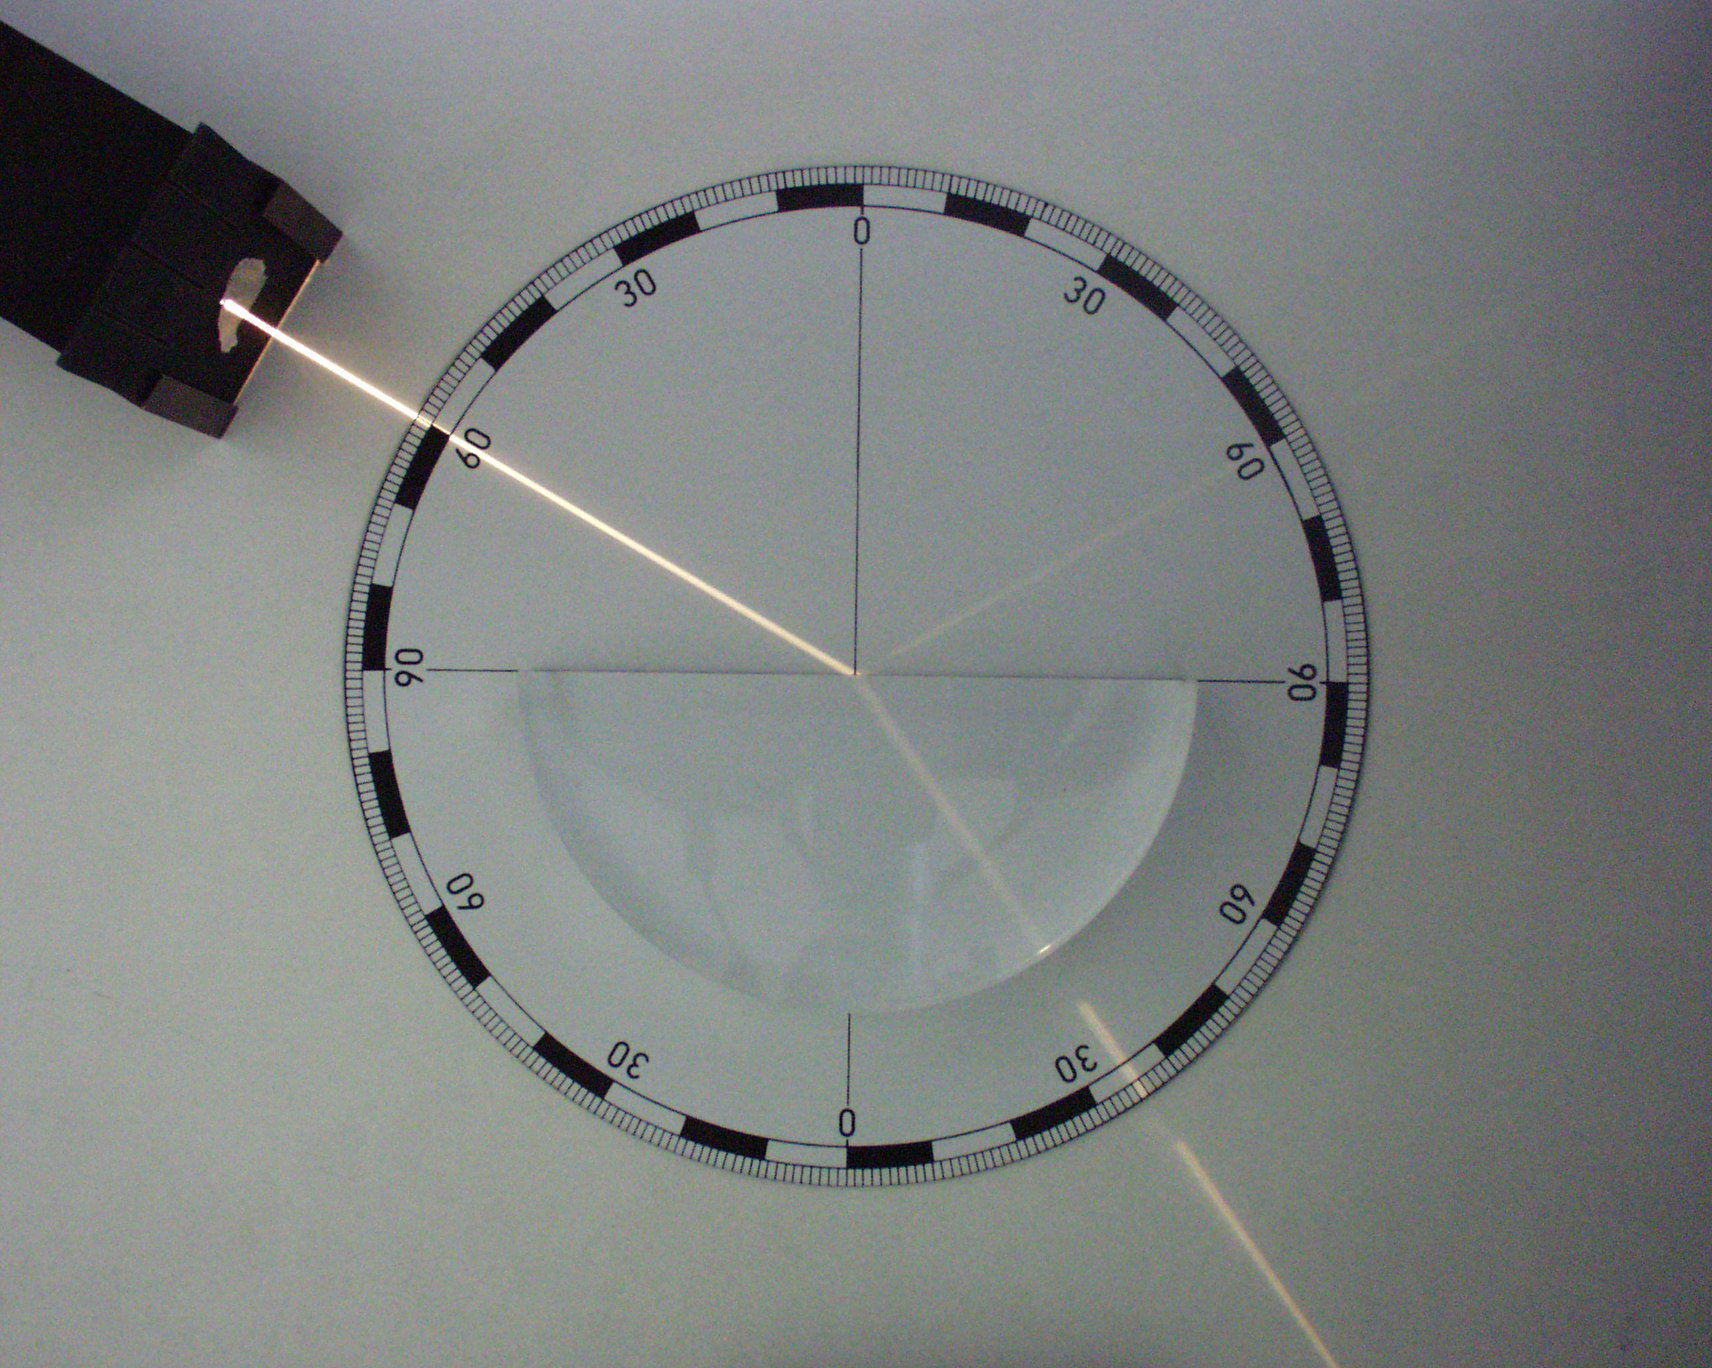
\includegraphics[width=\linewidth]{refraction_example.jpg}
  \caption{Refracción de un haz de luz.}
  \label{fig:refraction}
\end{wrapfigure}
Este cambio ocurre porque la velocidad de propagación de la onda no es la misma en distintos medios. Sin embargo, la frecuencia de la onda se conserva, lo cual implica que su longitud de onda cambia.

El índice de refracción \(n\) de un medio se define como:
\[
n = \frac{c}{v}
\]
donde:
\begin{itemize}
  \item \(c\) es la velocidad de la luz en el vacío.
  \item \(v\) es la velocidad de la onda en el medio.
\end{itemize}
Cuanto mayor es \(n\), más lento viaja la onda en ese medio.

\paragraph{Ley de Snell}

La dirección del rayo refractado está regida por la ley de Snell:
\[
n_1 \sin \theta_1 = n_2 \sin \theta_2
\]
donde:
\begin{itemize}
  \item \(n_1\), \(n_2\) son los índices de refracción de los medios 1 y 2.
  \item \(\theta_1\), \(\theta_2\) son los ángulos de incidencia y refracción medidos desde la normal a la superficie.
\end{itemize}

El límite o línea de separación entre los dos medios se llama frontera o interfaz.

\begin{figure}[ht]
  \centering
  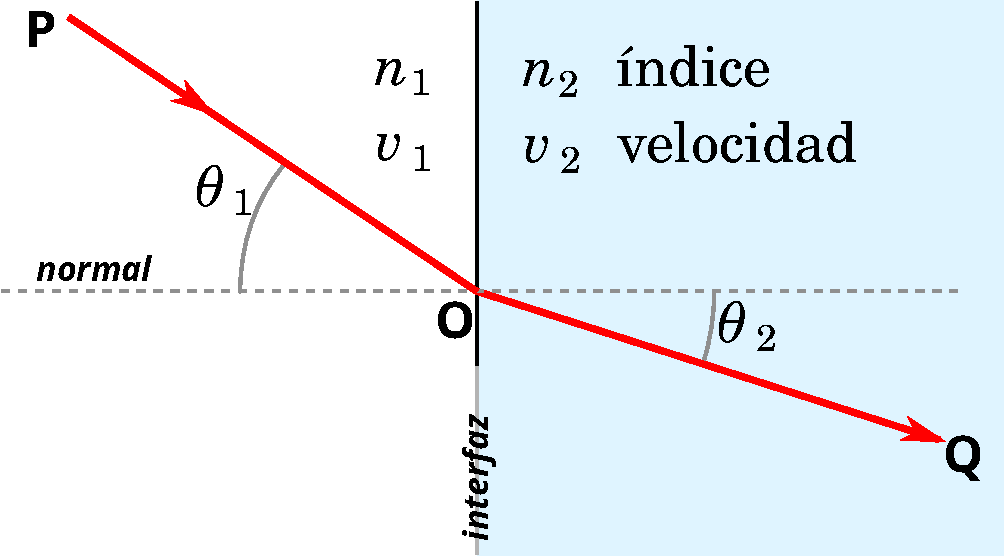
\includegraphics[width=0.5\textwidth]{snells_law.pdf}
  \caption{Ley de Snell.}
  \label{fig:snells_law}
\end{figure}

Cuando la onda cambia de medio la frecuencia \(f\) permanece constante (esto garantiza la continuidad temporal del campo eléctrico en la frontera), y la longitud de onda \(\lambda\) cambia según:
\[
\lambda_2 = \frac{v_2}{f} = \frac{c}{n_2 f}
\]
La dirección de propagación cambia si la onda incide oblicuamente.
\begin{itemize}
  \item Si \(n_2 > n_1\), la onda se desvía hacia la normal.
  \item Si \(n_2 < n_1\), se desvía lejos de la normal.
\end{itemize}
Sin embargo hay que tener en cuenta que existen casos especiales:
\begin{itemize}
  \item \textbf{Incidencia normal}: si la onda entra perpendicular a la superficie, no hay cambio de dirección, solo cambio en velocidad y longitud de onda.
  \item \textbf{Ángulo límite y reflexión total}: si la onda pasa de un medio más denso a uno menos denso y el ángulo de incidencia supera un cierto valor (ángulo crítico), no hay refracción, sino reflexión total interna.
\end{itemize}


\begin{wrapfigure}{r}{0.25\textwidth}
  \centering
  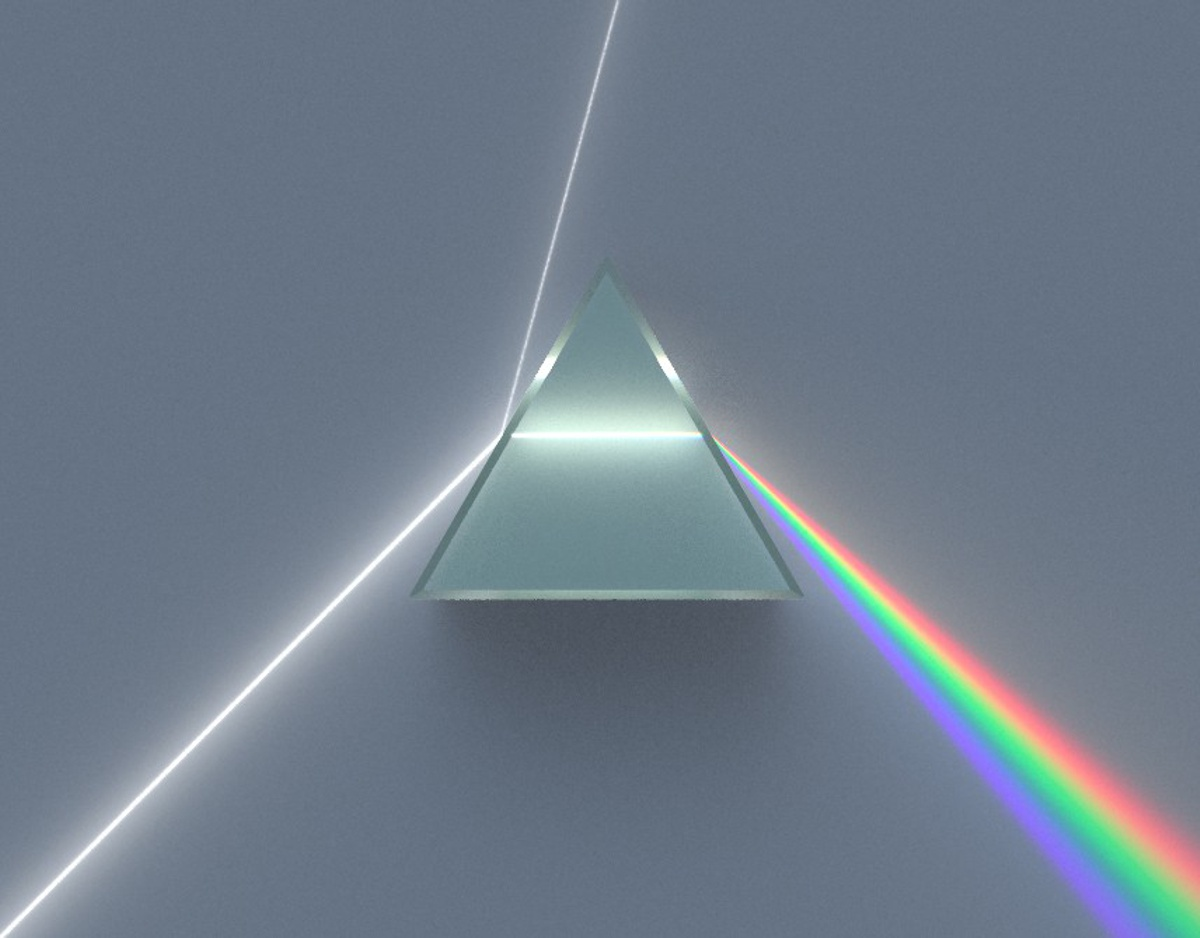
\includegraphics[width=\linewidth]{newton_prism.jpg}
  \caption{Dispersión de la luz en un prisma de Newton.}
  \label{fig:newton_prism}
\end{wrapfigure}
\paragraph{Dispersion de la luz}

En términos simples, la \textbf{dispersión de la luz} es el fenómeno por el cual la luz blanca se separa en sus distintos colores (como los del arcoíris) cuando pasa a través de un material, como un prisma o gotas de agua.

Esto ocurre porque cada color de la luz viaja a una velocidad ligeramente diferente dentro del material, lo que provoca que se refracten en ángulos distintos. Los colores con menor longitud de onda, como el violeta o el azul, se desvían más que los de mayor longitud de onda, como el rojo. Entonces cada color se refracta en un ángulo diferente, lo que hace que los colores se separen.

\subsubsection{Interferencia}

La \textbf{interferencia} es un fenómeno característico de toda onda, y se refiere a la superposición de dos o más ondas coherentes que se encuentran en un mismo punto del espacio, generando un resultado que puede ser de mayor o menor intensidad, según la fase relativa entre ellas.

En el caso de ondas electromagnéticas, como la luz, la interferencia se manifiesta en variaciones de intensidad debidas a la superposición del campo eléctrico de las ondas.

Cuando dos ondas electromagnéticas se superponen, los campos eléctricos (\(\vec{E}\)) se suman vectorialmente (principio de superposición):
\[
\vec{E}_{\text{total}} = \vec{E}_1 + \vec{E}_2
\]
La intensidad observada es proporcional al cuadrado del campo eléctrico resultante:
\[
I \propto |\vec{E}_{\text{total}}|^2
\]
Esto puede generar dos situaciones:
\begin{enumerate}
  \item \textbf{Interferencia constructiva}: los campos eléctricos están en fase (máximos con máximos, mínimos con mínimos), y la intensidad aumenta.
  \item \textbf{Interferencia destructiva}: los campos están en oposición de fase (máximo con mínimo), y la intensidad disminuye o se anula.
\end{enumerate}

\paragraph{Condiciones necesarias para que haya interferencia observable}
\begin{itemize}
  \item Coherencia temporal: Las ondas deben tener frecuencias iguales o muy similares.
  \item Coherencia espacial: Las ondas deben mantener una diferencia de fase constante en el tiempo.
  \item Polarización compatible: Las componentes del campo eléctrico deben estar alineadas o parcialmente alineadas.
  \item Superposición espacial efectiva: Las ondas deben encontrarse en una región del espacio donde sus frentes de onda se crucen.
\end{itemize}

\paragraph{Diferencia de fase y camino óptico}

El camino óptico es una magnitud que permite cuantificar el efecto que tiene un medio sobre la propagación de una onda electromagnética, en particular sobre su fase. Se define como el producto del índice de refracción del medio y la distancia recorrida por la onda en ese medio.
\[
L = n \cdot d
\]
donde:
\begin{itemize}
  \item $L$ es el camino óptico,
  \item $n$ es el índice de refracción del medio,
  \item $d$ es la distancia física recorrida en el medio.
\end{itemize}
El camino óptico representa la distancia que la luz habría recorrido en el vacío durante el mismo tiempo que tarda en recorrer una distancia \(d\) en un medio con índice \(n\). Por eso, es útil para comparar fases entre ondas que han atravesado distintos medios. Dos ondas que recorren diferentes caminos ópticos pueden llegar con distinta fase al punto de interferencia, lo que afecta si la interferencia es constructiva o destructiva.

Cuando dos ondas recorren diferentes medios o longitudes, se habla de diferencia de camino óptico:
\[
\Delta L = n_1 d_1 - n_2 d_2
\]
Esta diferencia está directamente relacionada con la diferencia de fase:
\[
\Delta \varphi = \frac{2\pi}{\lambda_0} \Delta L
\]
donde \(\lambda_0\) es la longitud de onda en el vacío.

Entonces, retomando la ecuación de la interferencia, para que la interferencia sea observada, la diferencia de camino óptico \(\Delta L\) entre las ondas determina la diferencia de fase \(\Delta \varphi\) siendo:
\begin{itemize}
  \item Constructiva si \(\Delta L = m \lambda_0\), con \(m \in \mathbb{Z}\) (en fase (\(m\,2\pi\)))
  \item Destructiva si \(\Delta L = (m + 1/2)\lambda_0\) (en fase contraria (\(m\pi\)))
\end{itemize}
Un ejemplo cotidiano es el fenómeno de interferencia en películas delgadas, como en burbujas de jabón o manchas de aceite, donde la luz se refleja en distintas capas.

Cuando la luz incide sobre una burbuja de jabón, parte de ella se refleja en la superficie exterior de la burbuja, mientras que otra parte se refleja en la superficie interior. Estas dos reflexiones de la luz se interfieren entre sí, produciendo un patrón de interferencia.

\begin{wrapfigure}{l}{0.24\textwidth}
  \centering
  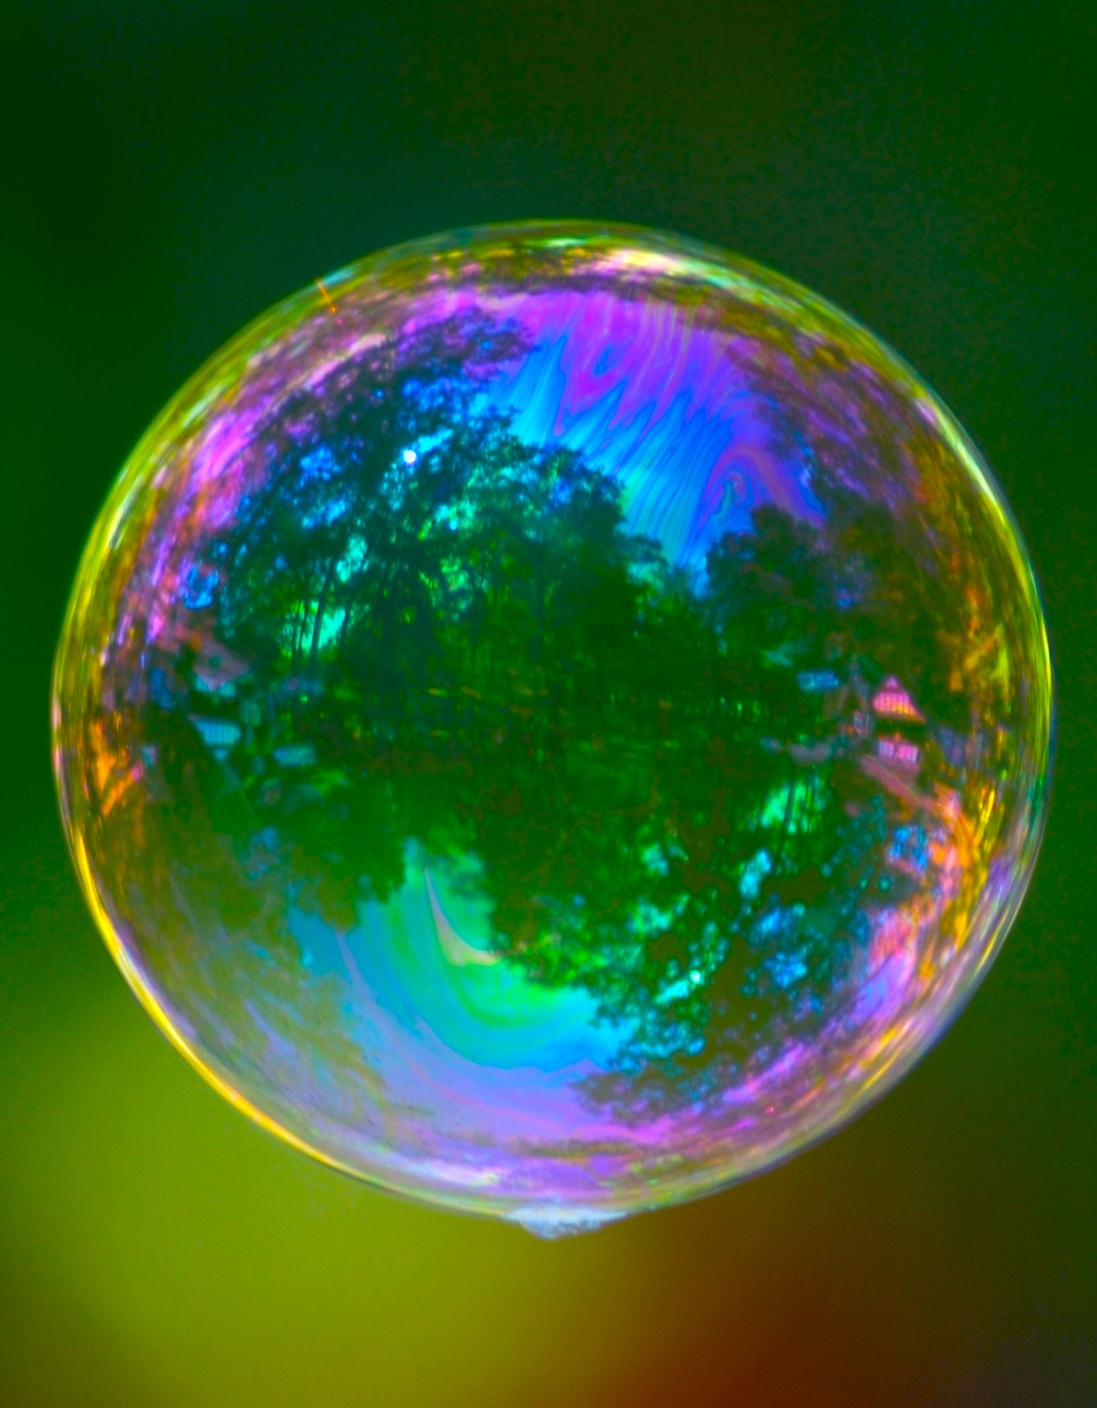
\includegraphics[width=\linewidth]{bubble.jpg}
  \caption{Patrón de colores en burbujas de jabón}
  \label{fig:burbujas_jabon}
\end{wrapfigure}
Dependiendo del grosor de la película de jabón, las ondas reflejadas en la superficie interior y exterior se encuentran en diferentes fases, lo que da lugar a diferentes patrones de interferencia. Esto hace que la burbuja parezca brillar con diferentes colores.

Específicamente, cuando las ondas reflejadas se encuentran en fase, se produce una interferencia constructiva y se observan colores brillantes. Cuando las ondas se encuentran en oposición de fase, se produce una interferencia destructiva y se observan colores más oscuros.

El grosor de la película de jabón varía continuamente a medida que la burbuja se expande y se contrae, lo que hace que los colores cambien constantemente. Esto crea el efecto de iridiscencia y el hermoso despliegue de colores que vemos en las burbujas de jabón.

Otro ejemplo típico de interferencia es el experimento de la doble rendija. Fue realizado por primera vez por Thomas Young en 1801. En este experimento, se hace pasar un haz de luz o de partículas subatómicas a través de una pantalla con dos rendijas paralelas. Detrás de la pantalla, se coloca una segunda pantalla donde se observa un patrón de interferencia.

Si la luz o las partículas se comportaran como partículas clásicas, se esperaría ver dos franjas brillantes en la segunda pantalla, correspondientes a las dos rendijas. Sin embargo, lo que se observa, como se ve en la figura \ref{fig:double_slit}, es un patrón de interferencia con franjas brillantes y oscuras, similar al patrón que se obtendría si la luz o las partículas se comportaran como ondas.


\begin{figure}[ht]
  \centering
  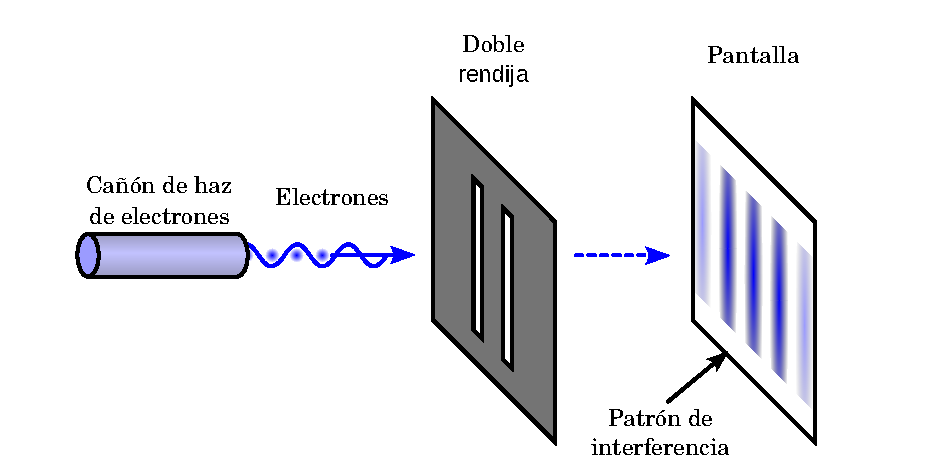
\includegraphics[width=0.75\textwidth]{double-slit.pdf}
  \caption{Interferencia de la luz por doble rendija}
  \label{fig:double_slit}
\end{figure}

\subsubsection{Difracción}

La \textbf{difracción} es un fenómeno ondulatorio que consiste en la capacidad de una onda de desviarse de su trayectoria rectilínea al encontrarse con un obstáculo o una abertura, propagándose luego en regiones que, según la óptica geométrica, deberían estar en sombra.

Este fenómeno es característico de todas las ondas, incluidas las ondas electromagnéticas como la luz, las microondas o las ondas de radio.

\begin{wrapfigure}{r}{0.25\textwidth}
  \centering
  \includegraphics[width=\linewidth]{water_difraction.jpg}
  \caption{Fenómeno de difracción en agua}
  \label{fig:water_difraction}
\end{wrapfigure}
Cuando una onda electromagnética incide sobre un obstáculo, parte de la onda puede rodearlo, por otro lado, si incide sobre una rendija o abertura, la onda puede expandirse desde la abertura en distintas direcciones, de la misma forma que lo hace el agua en la figura \ref{fig:water_difraction}.

Esto se debe a la naturaleza ondulatoria del campo electromagnético. No es que el campo ``decida'' rodear el obstáculo, sino que la propagación del campo obedece a principios físicos descritos por las ecuaciones de Maxwell y la teoría de Huygens-Fresnel.

Como vimos en la introducción, el principio de Huygens-Fresnel establece que:

``Cada punto de un frente de onda se comporta como una fuente secundaria de ondas esféricas. La onda total en cualquier región del espacio es la superposición de todas estas ondas secundarias.''

Entonces, cuando una onda electromagnética encuentra una rendija o el borde de un obstáculo cada punto del borde actúa como una fuente secundaria, estas ondas secundarias se interfieren, generando un nuevo frente de onda que se curva y se propaga más allá del borde.

\paragraph{Condición para observar difracción significativa}

La difracción es más pronunciada cuando el tamaño de la abertura u obstáculo \(a\) es comparable a la longitud de onda \(\lambda\):
\[
a \approx \lambda
\]
Por ejemplo:
\begin{itemize}
  \item La luz visible (con \(\lambda \sim 500 \text{ nm}\)) se difracta notablemente en rejillas o rendijas microscópicas.
  \item Las ondas de radio (con \(\lambda \sim \text{m}\)) pueden difractarse alrededor de montañas o edificios, lo que permite su recepción en zonas sin línea de vista.
\end{itemize}

Un ejemplo de el fenómeno de difracción es el patrón de difracción de una rendija única. Una fuente de luz monocromática pasa por una rendija estrecha y se produce un patrón de franjas por difracción e interferencia.

\begin{figure}[ht]
  \centering
  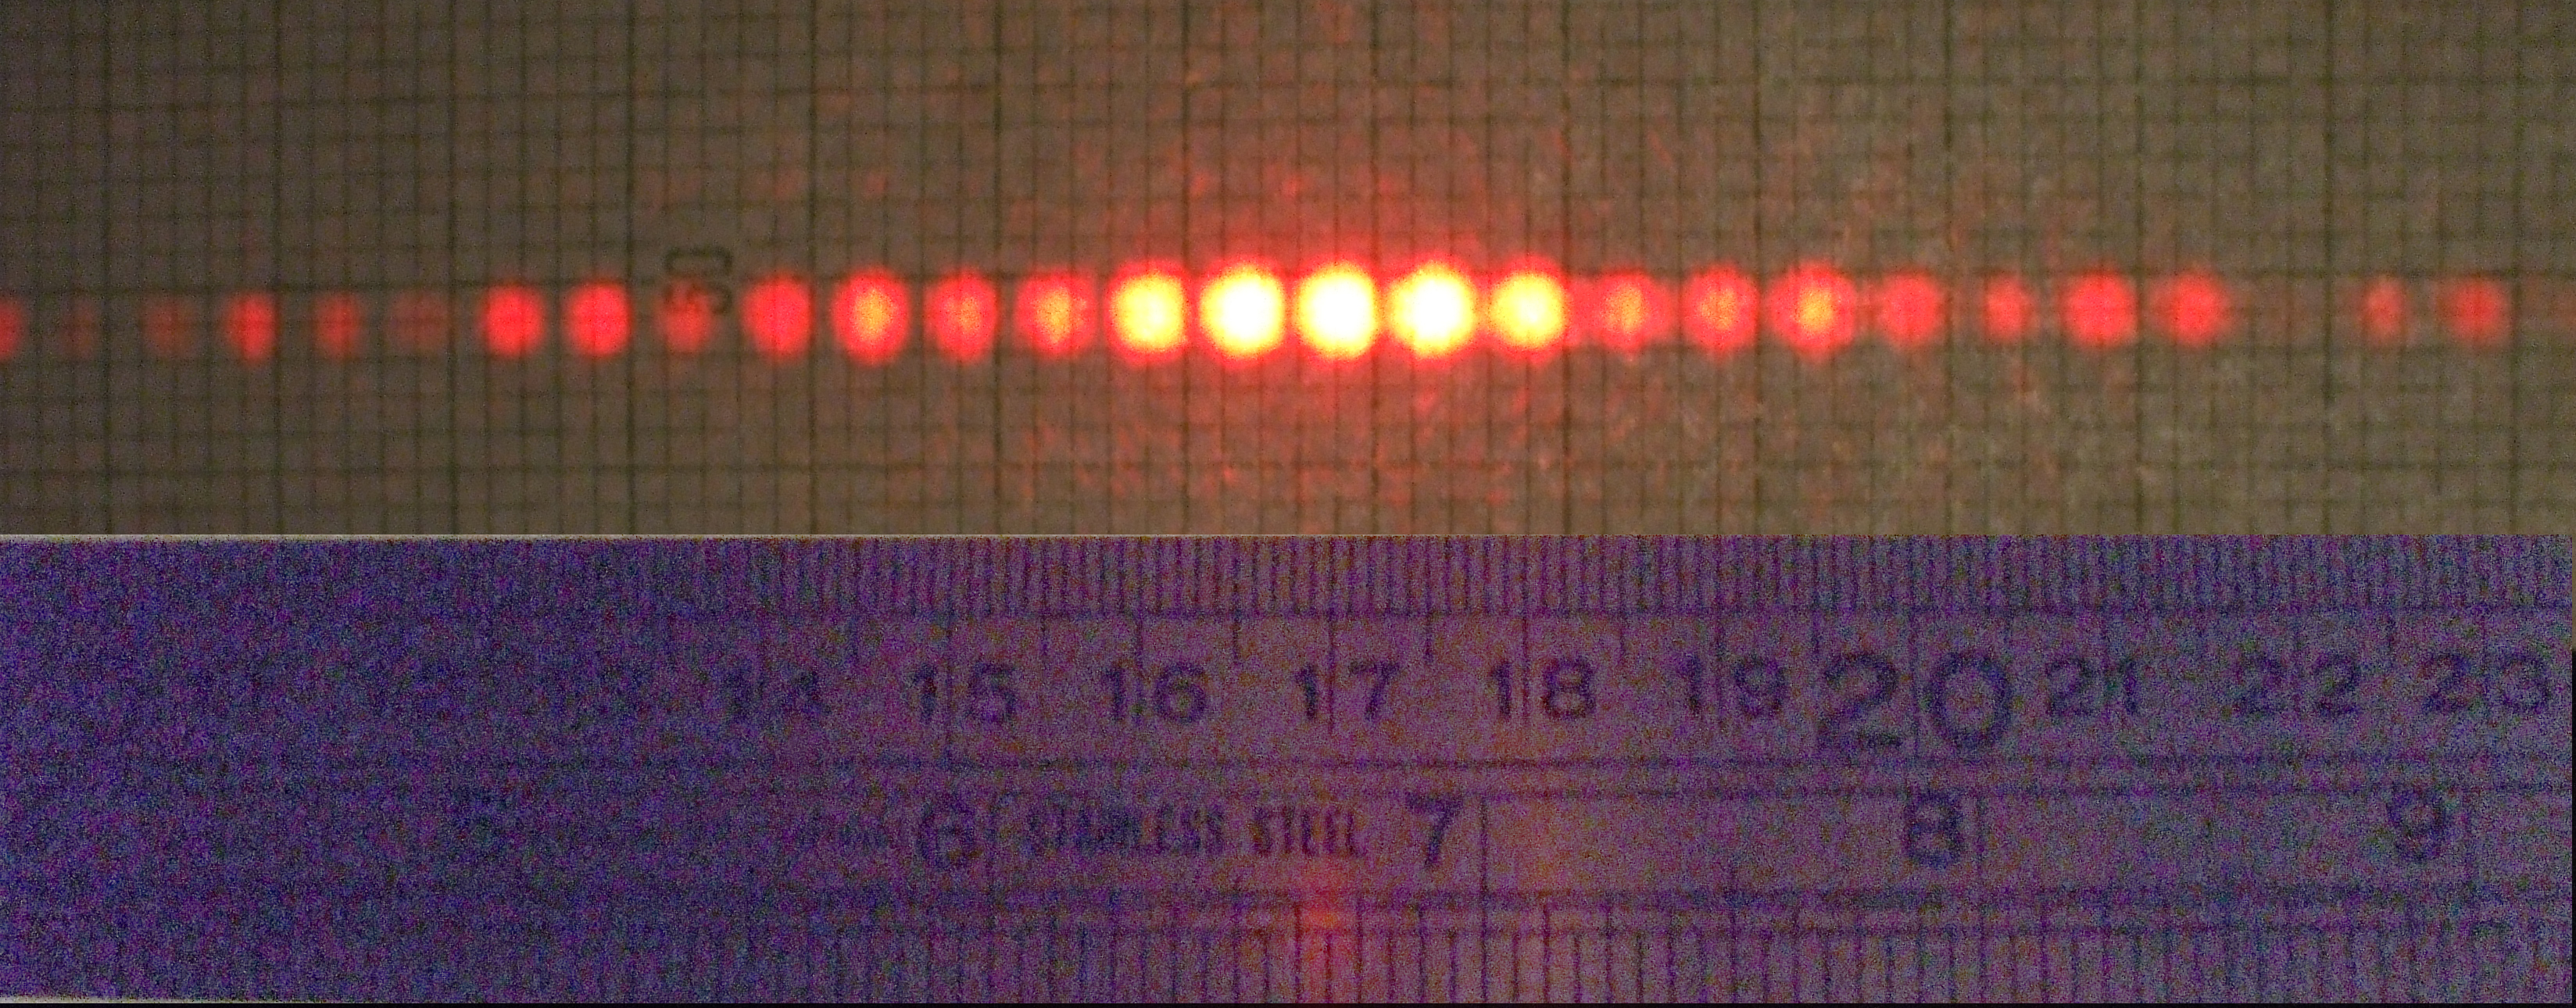
\includegraphics[width=0.75\textwidth]{diffraction_150_slits.jpg}
  \caption{Patrón de difracción de un haz de luz de 633nm por múltiples rendijas. Foto de: \href{https://commons.wikimedia.org/w/index.php?curid=6938945}{Shim'on y Slava Rybka (Wikipedia)}.}
  \label{fig:diffraction_150_slits}
\end{figure}

En la imagen \ref{fig:diffraction_150_slits} se puede ver que hay una serie de franjas brillantes y oscuras, que son los patrones de interferencia constructiva y destructiva, respectivamente. Es importante que no confunda esto con el ejemplo de una sola rendija. Si bien se producirá el fenómeno de difracción, no se producirá interferencia constructiva, ya que no hay una segunda fuente de luz. La forma que tendríamos de detectar que se ha producido difracción es encontrar que la luz se encuentra en regiones que, según la óptica geométrica, deberían estar en sombra.

\subsubsection{Polarización}

La polarización es la orientación de la vibración de una onda transversal en un solo plano. Solo ocurre con ondas transversales, como la luz; no ocurre con ondas longitudinales como el sonido.

\begin{wrapfigure}{r}{0.38\textwidth}
  \centering
  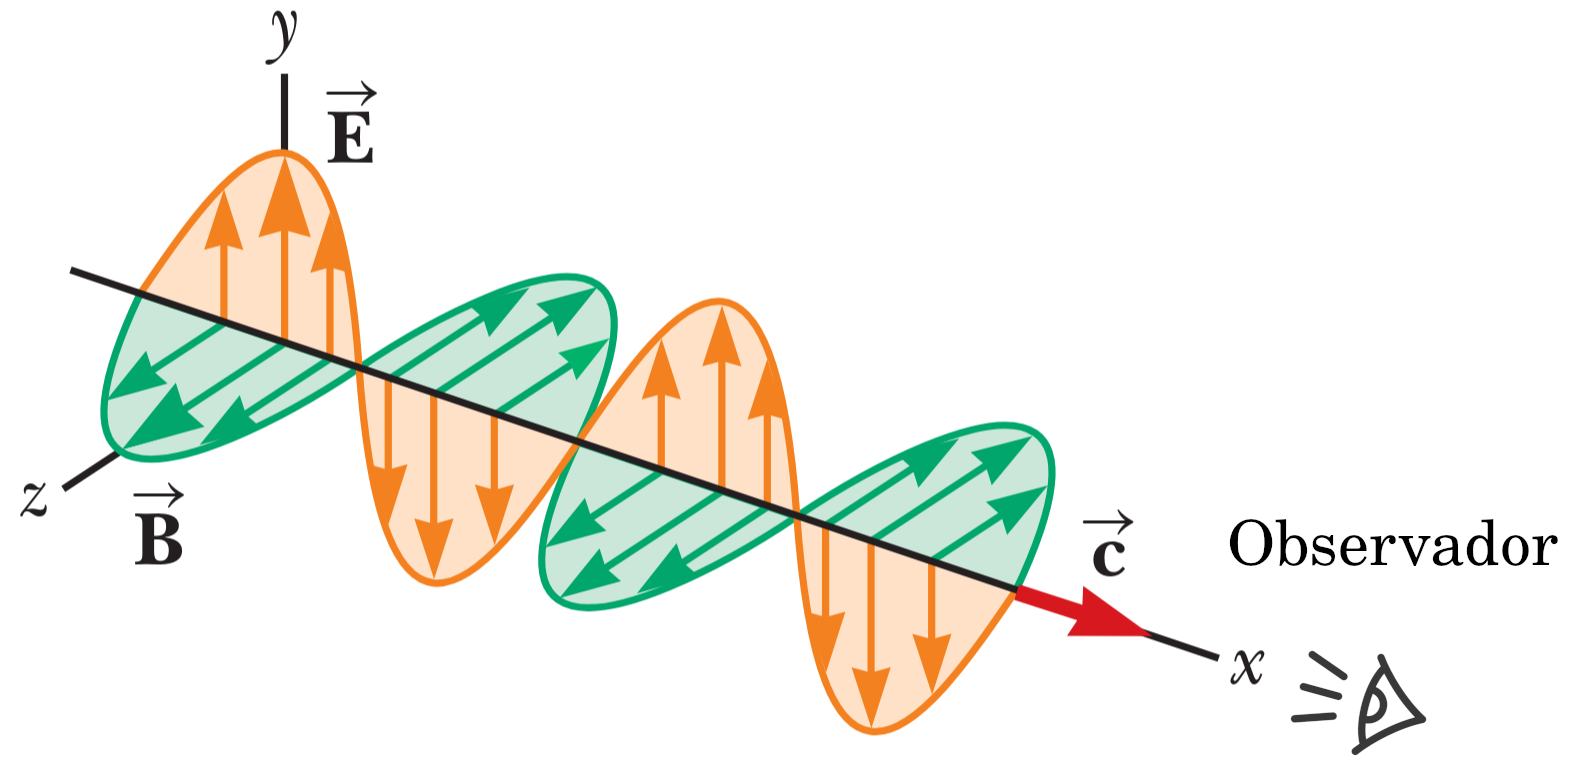
\includegraphics[width=\linewidth]{polarization_observer.png}
  \caption{Posición del observador con respecto a la onda electromagnética.}
  \label{fig:polarization}
\end{wrapfigure}
Para ondas electromagnéticas en general, \textbf{polarización} es el fenómeno ondulatorio por el cual se restringe o determina la dirección de oscilación del campo eléctrico de una onda electromagnética. Recuerda que una onda electromagnética está compuesta por dos campos perpendiculares entre sí y a la dirección de propagación: el campo eléctrico \(\vec{E}\) y el campo magnético \(\vec{B}\) como se vió anteriormente. Ahora supongamos una onda electromagnética como la de la figura \ref{fig:polarization}, donde la propagación de la onda es en la dirección \(x\) y hay un observador mirando sobre el eje \(x\) hacia el origen.

La \textbf{dirección de polarización} se define convencionalmente como la dirección del \hl{campo eléctrico}. Entonces, el observador de la figura \ref{fig:polarization} verá que la onda electromagnética está polarizada en la dirección \(y\). Digamos, vería un vector \(\vec{E}\) que oscila en la dirección \(y\).

Las ondas electromagnéticas naturales (como la luz solar) están compuestas por muchas ondas con diferentes orientaciones de \(\vec{E}\) emitidas por los átomos de la fuente luminosa. Cada átomo produce una onda que tiene una orientación particular, por lo que se dice que están \textbf{no polarizadas}. El ojo humano no puede distinguir entre ellas, únicamente es capaz de distinguir la intensidad de la luz, por lo que el observador de la figura \ref{fig:polarization} supondremos que es capaz de distinguir la polarización de la luz.

Cuando se polarizan las ondas electromagnéticas, se pueden obtener diferentes tipos de polarización.
\begin{itemize}
  \item \textbf{Polarización lineal}: el campo eléctrico oscila en una sola dirección fija perpendicular a la dirección de propagación.
  \item \textbf{Polarización circular}: la punta del vector \(\vec{E}\) describe un círculo en el plano perpendicular a la dirección de propagación. Esto ocurre cuando dos componentes perpendiculares del campo eléctrico tienen igual amplitud y desfasaje de \(\pi/2\).
  \item \textbf{Polarización elíptica}: generalización de la circular, donde las componentes tienen diferente amplitud y/o fase, formando una elipse.
\end{itemize}
Si deseas ver gráficamente los distintos tipos de polarización recomiendo ver el siguiente video: \href{https://www.youtube.com/watch?v=PMjADwpLlfs}{Polarización de la luz (Khan Academy) | YouTube}.

\paragraph{¿Cómo se produce la polarización?}
\begin{itemize}
  \item \textbf{Por filtrado}: usando un polarizador (como un cristal de polaroide) que solo permite pasar la componente del campo eléctrico en una dirección específica.
  \item \textbf{Por reflexión}: al reflejarse en una superficie, la luz puede quedar parcialmente o totalmente polarizada, especialmente en el ángulo de Brewster.
  \item \textbf{Por dispersión}: como en el cielo, donde la luz solar se dispersa al interactuar con las moléculas del aire, generando polarización.
\end{itemize}

\paragraph{¿Solo el campo eléctrico se ve afectado en la polarización?}

Sí, en términos de definición y observación, solo el campo eléctrico se considera en la descripción de la polarización.

Esto se debe a que el campo eléctrico es el responsable de la interacción con la materia, como con sensores ópticos o el ojo humano. El campo magnético \(\vec{B}\) está siempre perpendicular al campo eléctrico y a la dirección de propagación, por lo tanto, su dirección queda automáticamente determinada una vez que se fija la del campo eléctrico.

En otras palabras, al definir la polarización, no es necesario especificar el campo magnético porque este está completamente determinado por la dirección del campo eléctrico y la dirección de propagación.